\begin{frame}[fragile]

  \frametitle{Programmation}

\begin{tabular}{p{0.35\textwidth}|p{0.55\textwidth}}
\begin{minipage}[t]{\linewidth}
  \begin{lstlisting}[]
;Fibonacci Binaire
  0111001000
  0000000001
  0000010000


  0001011000
  1001001000
  0011010000

  0111101000
  0000000011
  \end{lstlisting}

\end{minipage}&\begin{minipage}[t]{\linewidth}
  \begin{lstlisting}[]
;Fibonacci Assembleur
	MOV A 1 	;mettre 1 dans A

	MOV B 0		;mettre 0 dans B

boucle :
	MOV C A   	  ;A dans C
	ADD A      	  ;A + B dans A
	MOV B C   	  ;C dans B

	MOV PC boucle ;revenir a 'boucle'
  \end{lstlisting}
\end{minipage}
\end{tabular}

  \begin{lstlisting}[language=Python]
#Fibonacci Python
a = 1
b = 0

while (True) : #(pas de condition d'arret)
	c = a
	a = a + b
	b = c
  \end{lstlisting}



\end{frame}




\begin{frame}

  \frametitle{Simulation}


  \begin{figure}

    \centering
    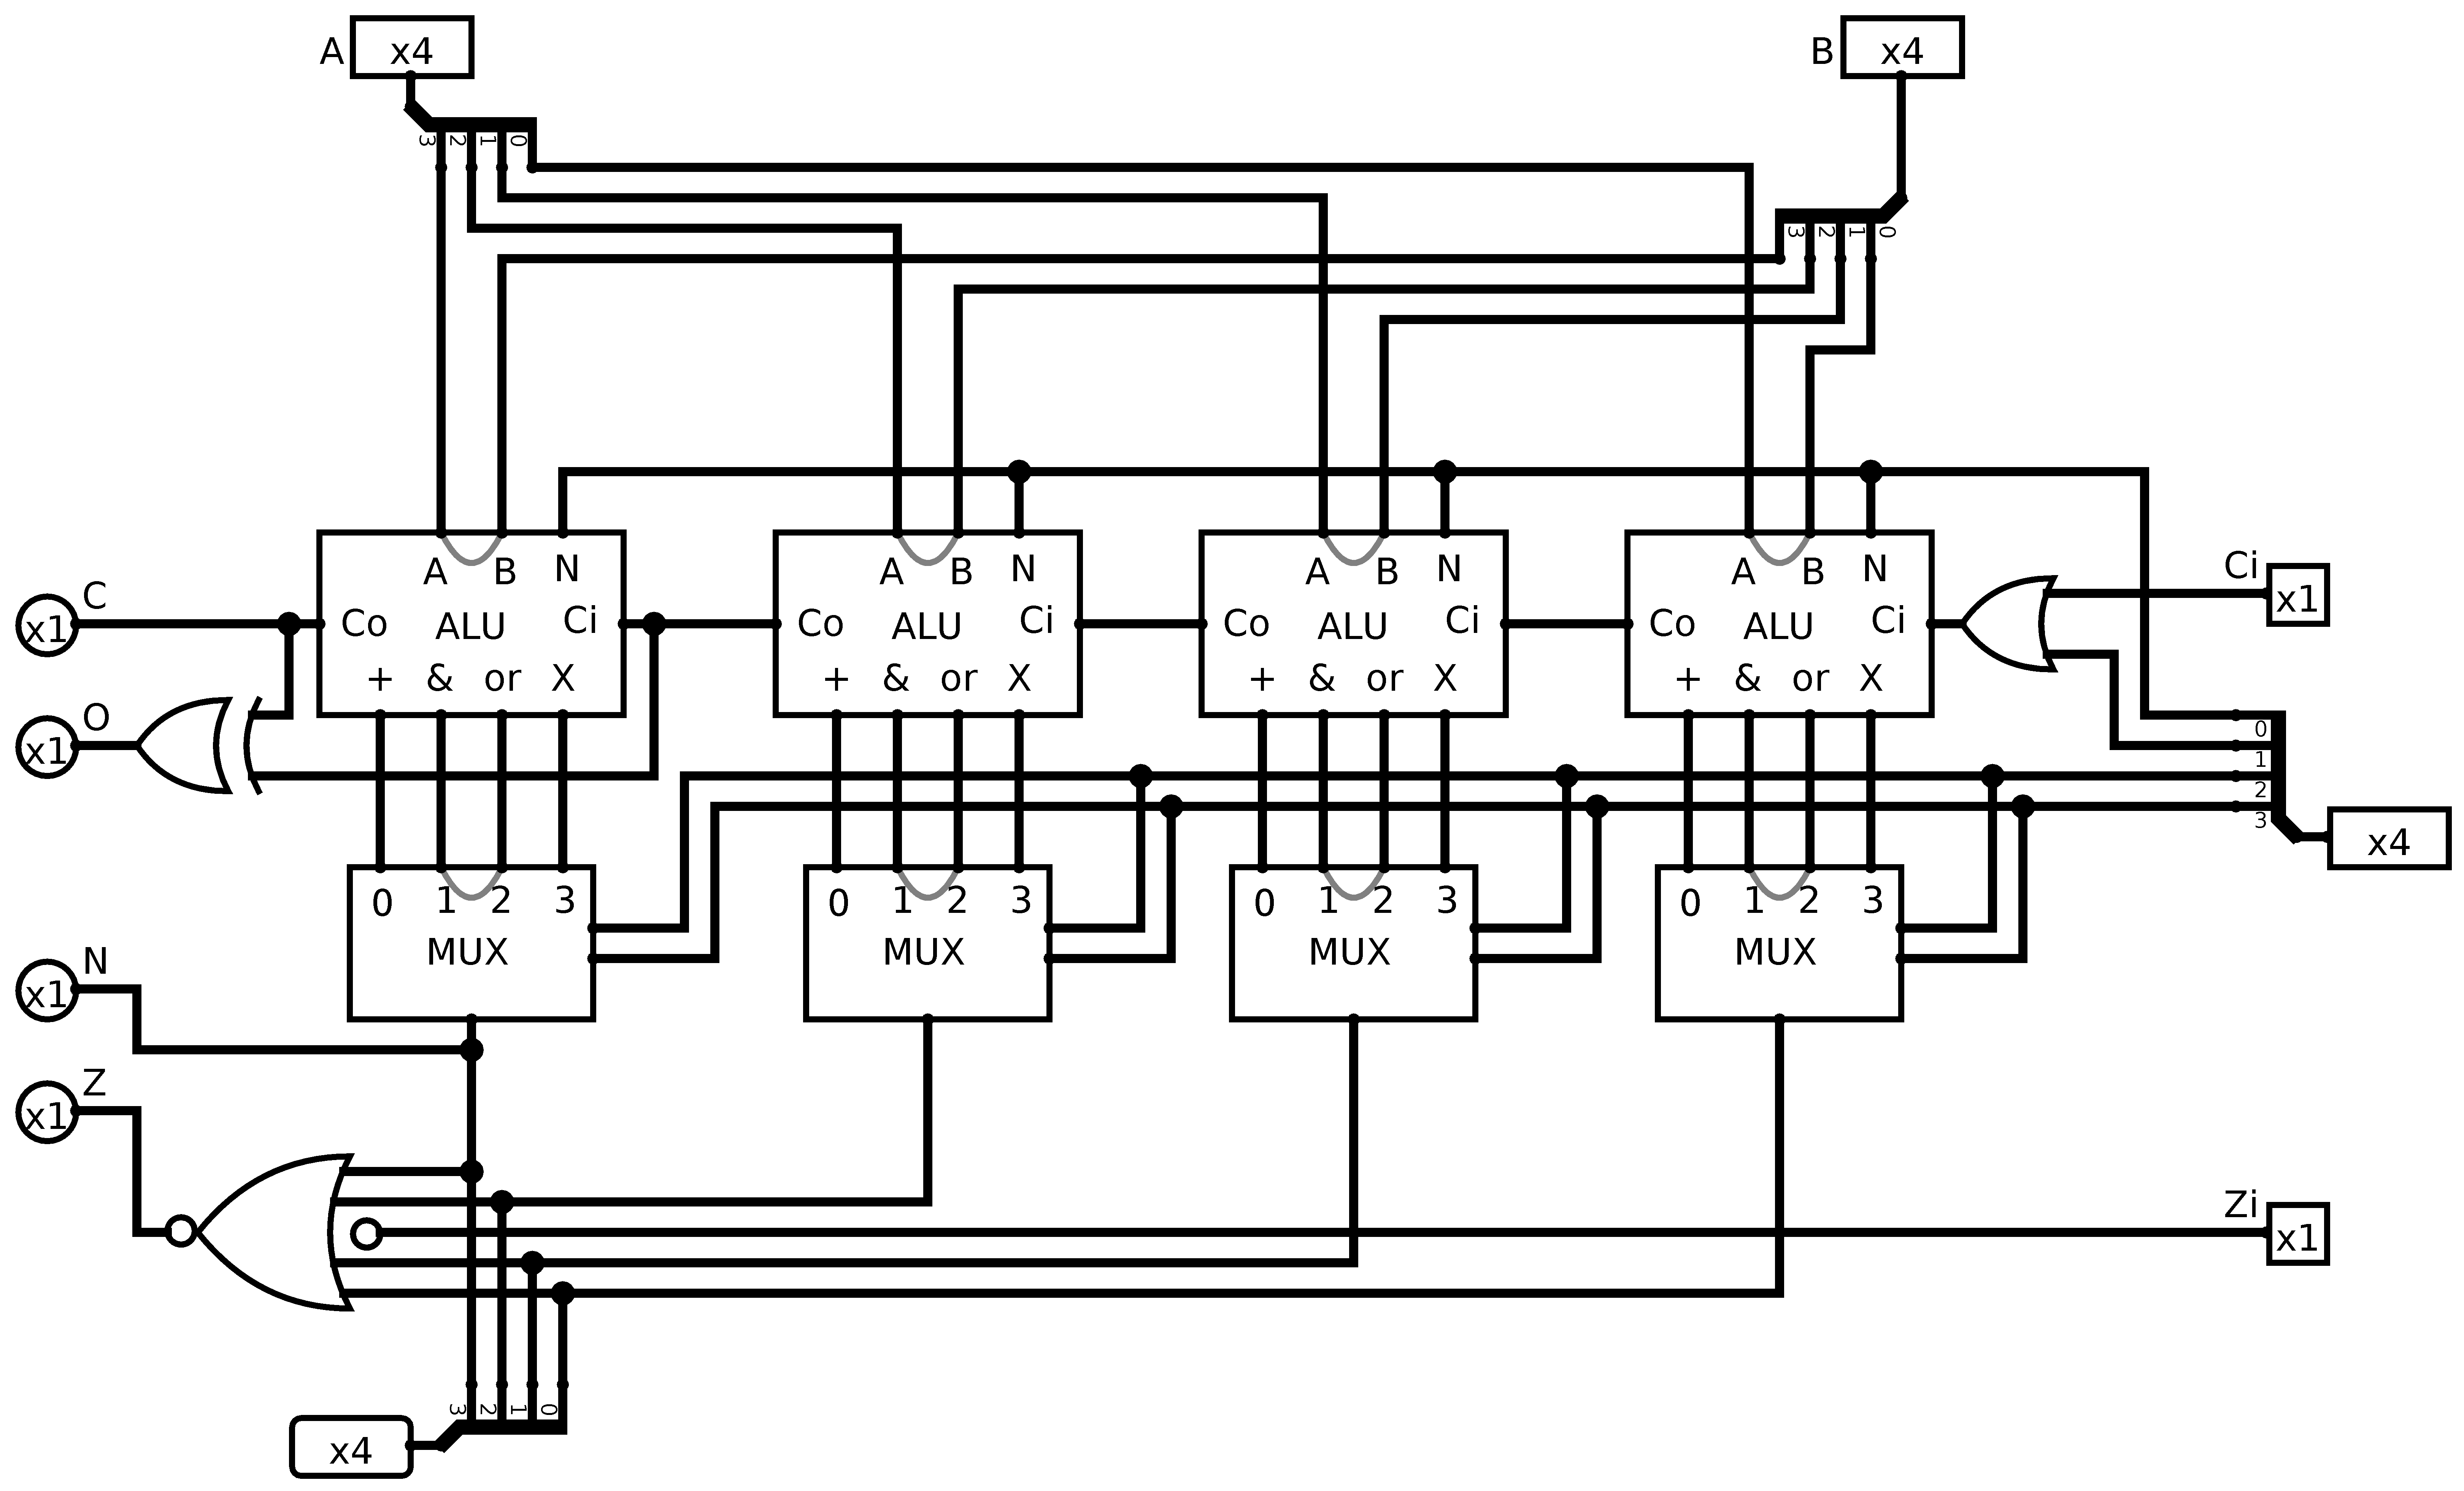
\includegraphics[width=\linewidth]{pics/test.png}

  \end{figure}


\end{frame}
